% This program is free software: you can redistribute it and/or modify
% it under the terms of the GNU General Public License as published by
% the Free Software Foundation, either version 3 of the License, or
% (at your option) any later version.

% This program is distributed in the hope that it will be useful,
% but WITHOUT ANY WARRANTY; without even the implied warranty of
% MERCHANTABILITY or FITNESS FOR A PARTICULAR PURPOSE.  See the
% GNU General Public License for more details.

% You should have received a copy of the GNU General Public License
% along with this program.  If not, see <http://www.gnu.org/licenses/>.


% NOTE:
% htlatex tips.tex
% graphics file must be in the format of .eps
% htlatex $(file_name).tex "html, 4, mouseover, frames, next" "" "-dweb/"
% htlatex tips.tex "html, 1, mouseover, next"

\documentclass{report}

\usepackage{mystyle}

\title{R 튜토리얼 \\ - Some R Problems Derived Me Nuts! -}
\author{iHELP Working Group}
\date{\today}

\begin{document}
\maketitle

\chapter{서문}

\texttt{R}을 사용하게 된 이래로 여러가지 경험들을 바탕으로 도움이 되고자 하는 내용을 정리하는 페이지입니다.
% 이 문서의 작성자 역시 다른 사용자들의 똑똑한 테크닉들을 항상 배우고 있습니다.

본 페이지는 다양한 종류의 패키지들을 활용하는 방법보다는 \underline{R 기본 시스템에서 제공되어진 기능들만을 이용하여 원리중심의 문제해결을 돕기 위한 내용들만을 정리하려고 노력중입니다}. 
이 문서는 매일 갱신이 되며, 문서의 최초 작성일은 2013년 4월 10일입니다.

만약, 이 페이지를 읽고 있는 사용자가 이 문서가 도움이 되었다고 생각된다면 문서에 더 많은 내용이 기재될 수 있도록 추가, 수정 및 제안에 대한 내용을 \href{mailto:ihelp-urquestion@lists.r-forge.r-project.org}{ihelp-urquestion@lists.r-forge.r-project.org}의 주소로 이메일을 보내주시길 부탁드립니다. 

\textbf{\underline{본 페이지는 iHELP Working Group의 관리자에 의해서 정리가 되고 있지만, ihelp-urquestion 메일링 리스트를 활용하시는 사용자님들의 도움을 통하여 확장되고 있습니다.
이 문서의 작업에 도움을 주신 분들은 아래와 같습니다}}. 

\begin{itemize}
	\item Chel Hee Lee
	\item Eugene Jung 
	\item Jong Hwa Shin
\end{itemize} 

메일링에 등록된 내용은 이 문서의 관리자가 문서를 갱신할 때마다 반영하도록 노력할 것입니다.

\begin{enumerate}
	\item (제안) 본 페이지 자체를 데이터 분석을 위한 프로세스를 나타낼 수 있도록 섹션구성 자체를
	\begin{itemize}
		\item 최초 데이터의 입력과 확인 
		\item 데이터를 조작
		\item 데이터 정리하기 
		\item 통계로 데이터를 설명하기 
		\item 그래픽적으로 보여주기 
		\item 원하는 그래픽 만들기
	\end{itemize}
	으로 조정함. -- 즉각적 수용 -- 문서구조 변경함 (2013-APR-24)
\end{enumerate}

%%%%%%%%%%%%%%%%%%%%%%%%%%%%%%%%%%%%%%%%%%%%%%%%%%%%%%%%%%%%%%%%%%%%%%%%
%
% Data Management
%
%%%%%%%%%%%%%%%%%%%%%%%%%%%%%%%%%%%%%%%%%%%%%%%%%%%%%%%%%%%%%%%%%%%%%%%%

\chapter{미분류 질문들}
이 섹션에 등록된 질문들은 접수만 되고 아직은 답변되지 않은 상태입니다
% http://www.columbia.edu/~cjd11/charles_dimaggio/DIRE/resources/R/rFunctionsList.pdf
% http://www.ats.ucla.edu/stat/r/library/advanced_function_r.htm
% http://www.sr.bham.ac.uk/~ajrs/R/r-function_list.html
% http://www.scidav.org/techno/r_environments


% 이런 느낌은 특히 최소한 내가 알기로는 경영학과 경제학 분야(거의 확실함) 및 사회학, 심리학 분야가 특히 심하다. 
% 그리고 이들 분야에서는
% R의 다양한 기능(특히 visualization) 또는 packages를 필요로 하지 않을 가능성이 높다. 왜냐하면 분석 방법이 단순하기 때문이다.
% 여기에서 분석 방법이 단순하다는 것은 그 이론적 배경이 쉽다는 것을 의미하는 것이 아니라 절차상의 얘기이다.
% 언급한 분야에서 학술연구에서 실행되는 분석의 양을 보면 대부분 [기술통계 - 상관관계 - 차이분석, 회귀분석, 구조방정식분석] 정도로
% 분석이 마무리 되기 때문이다. 그리고 대부분 표(table)로 결과를 보고하는 형식을 따르고 있다.
% 분석 모형 자체를 다루는 연구가 거의 없는 것이다. 따라서 R의 작업 방식은 그들에게는 불필요할 지도 모른다.

% 그러나 여전히 R의 다양한 source를 필요로 하는 아주 작은 규모의 학술연구 분야는 존재한다. 따라서 여기의 tips에는 이들을 고려하여
% R 사용에 도움이 될 만한 사항들을 정리하고자 한다.
% 개인적으로는 통계학 및 다른 분야의 연구 과정이 어떻게 진행되는지 잘 모르는 것도 한 몫하여 이에 해당하는 부분은 다른 이의 도움이
% 절실하다.

% 덧붙여 나는 윈도우 환경에서의 R tip에 주목하고자 한다(Mac이나 유닉스/리눅스 환경에서의 R 사용에 관한 tip도 다른 이의 도움이 필요한
% 부분이다). 그 이유는 내가 윈도우에서 SPSS와 SAS를 숙련시켜 왔기 때문에 대부분의 통계분석 초심자들도 윈도우 환경에서 R 을 접하게
% 될 것이라는 막연한 억측 때문이다. 시간이 지나면서 여러 사람들을 만나보게 꼭 그렇지만은 않다는 것을 알게 되었지만 최소한 경영학과
% 경제학 분야에 속한 사람들은 그럴 것이라는 확신 때문이다. 이것은 다른 분야의 사람들을 홀대하는 것이 아니라 나의 능력의 한계 때문이다.
% 실제로 나의 경우에도 최근에 C 언어, CentOS, 그리고 MySQL도 공부하기 시작했으니 오해는 하지 말기 바란다(누군가는 포기하라고도 했다.
% 왜냐하면 지금 그것들을 공부하기에는 분량이 너무 많고 난이도가 낮지 않기 때문이다). 그런데 결국에는 내 전공분야에서의 R 사용은
% 그 분량이 많지 않고 리눅스/유닉스 기반의 R 사용에 보다 많은 시간과 지면을 할애하게 될 것이라는 생각이 든다.

% R은 최근의 빅데이터라는 화두와 함께 큰 주목을 받고 있다. 하지만 대부분의 사람들, 특히 사회과학 전공자들은 이 개념적 정의도 제대로
% 알지 못하며 들어보지 못한  전문용어(SQL, Hadoop, 그리고 Mapreduce 등)에 혹하고 있는 실정이다.
% 나의 경우 R을 구글링(googling)으로 공부하였다. 왜냐하면 내가 재학하던 대학에서는 R 교육 프로그램이 없었기 때문이다. 처음 접하게 된
% 것은 미시경제분석 수업이었다. 그 수업에서 교수님이 수업을 진행하시는데 R을 사용한 것이다(SAS도 조금 사용했었으나 SPSS 는 잡동사니
% 취급을 하셨던 것으로 기억한다). 누군가에게 강의를 받는 식의 교육은 그것이 전부였다. 이후의 학습은 모두 맨땅에 해딩과 계란으로
% 바위깨기 식이었다. 이 R tips 과정은 이러한 어려움을 덜어주기 위한 방안이 될 수도 있을 것이다.
% 그러기를 한참 후 어느 정도 익숙해지고 나니, 또 연구자로서의 건방이 살아나 R 교육이 어떻게 이루어지고 있는 지가 궁금해졌다.
% 이 부분은 나중에 다시 써 볼라오,,,
\begin{enumerate}
	
% 아래의 주소로부터 질문 다 만들어내기 	
% http://www.statmethods.net/input/valuelabels.html


	
	
	\item 데이터의 형변환과 결측치에대 대한 전반적인 내용을 알려주면 될 듯함.

	\item 기본 데이터 형에 대해서 -- 벡터, 행렬, 배열, 데이터 프레임, 리스트, 요인, 그리고 이들을 다루는데 필요한 함수들 
	% http://www.statmethods.net/input/datatypes.html
	\begin{Schunk}
	\begin{Soutput}
	ls()

	names(mydata)

	str(mydata)


	dim(object)

	class(obj)

	mydata

	head(mydata, n=10)

	tail(mydata, n=5) 

	length(obj)
	str(obj)
	class(obj)
	names(obj)
	
	c(obj,obj,...)
	cbind(obj, obj, ...)
	rbind(obj, obj, ...)
	
	obj
	
	ls()
	rm(obj)
	
	newobject <- edit(obj)
	fix(obj)
	\end{Soutput}
	\end{Schunk}
% 	levels(mydata$v1)


	\item 데이터 입출력 
	% http://www.statmethods.net/input/importingdata.html
	\begin{Schunk}
	\begin{Soutput}
	mydata <- read.table("c:/mydata.csv", header=TRUE, sep=",", row.names="id")
	write.table(mydata, "c:/mydata.txt", sep="\t") 
	\end{Soutput}
	\end{Schunk}
	\item R을 사용하기 전에 반드시 알아두어야 할 점 -- R은 모든 연산을 열벡터를 기준으로 한다는 것을 반드시 알고 시작해야 함.  SAS는 행벡터임.  따라서, 가끔 R에서 벡터사이즈가 어쩌구 할때는 바로 데이터의 수가 R이 해결하기에는 부족하다는 점이다.  그런데, 어떤 경우 이것은 주로 메모리 조절과 관계가 있음. 
	
	\item (접수: 2013-APR-23)  NA 와 NaN을 데이터로부터 찾고 싶어요.
	
	\textsf{(답변)} 요것은.... \texttt{is.na()}와 \texttt{is.nan()} 함수 사용법을 알려주면 좋음.  추가로 \texttt{is.null()}도 알려주면 \texttt{is}관련 함수들에 설명해주면 짱임.
	
	\item (접수: 2013-APR-23)  분기문 쓸때요 \texttt{if}문 사용하는 것은 알고 있습니다.  그런데, C 언어처럼 중간에 루프를 완전히 끊고 나가는 방법이 있거나 혹은 해당 루프를 넘어가는 방법이 있나요?  예를들면, Basic 언어에서 보면 goto 같은 것도 있는지 알고 싶어요.
	
	\textsf{(답변)} 요건... 질문이 좀 방대한건데... \texttt{repeat}, \texttt{while}에 대해서 간단히 보여주고, \texttt{break}과 \texttt{next} 를 알려주면 좋음. 
	만약, 메시지 역시 설명해줄려면  \texttt{stop()}, \texttt{warning()}도 함께 설명해주면 최고임.  

	\item (접수: 2013-APR-23)  저는 다각형을 그리고 싶습니다. 
	
	\textsf{(답변)}  이것은 간단히 2차원-랜덤포인트 생성한 뒤에 \texttt{polygon()} 함수를 써서 보여주면 됨. 

	\item (접수: 2013-APR-23)  제가 가진 데이터셋이 있는데, 이 데이터를 어떤 특정한 변수들의 값을 이용하여 분류하려고 합니다.  어떻게 해야하나요?
	
	\textsf{(답변)}  요것은 \texttt{split()} 함수를 이용하도록 알려줄 것. 

	\item (접수: 2013-APR-23) 제가 가진 데이터 프레임에 NA 값들이 있는데, NA 때문에 분석이 이상해지는 것 같아, NA를 가진 데이터 행자체를 없애고 싶습니다.  한번에 해주는게 없나요? 
	
	\textsf{(답변)}  요건 \texttt{na.omit()}과 같은 함수를 이용하는 법을 알려줄 것.  흠.. \texttt{na.action}이라는 개념을 알려주면 더욱 좋음. 

	\item (접수: 2013-APR-23) 논리형 벡터가 있는데, 이 벡터의 구성요소가 모두 TRUE 인지 알고 싶습니다. 
	
	\textsf{(답변)} 이건 \texttt{isTRUE()}함수와 \texttt{all()}함수를 통해 알려주면 매우 좋음.
	
	\item (접수: 2013-APR-23) t-테스트 하는 방법 좀 알려주세요 -- 통계적 해석을 덧 붙여주시면 좋을 것 같습니다.
	
	\textsf{(답변)} \texttt{t.test()} 함수 사용법을 알려줄 것 -- 일반화 된 옵션 다 알려주면 더 좋을 것 같음. 
	
	\item (접수: 2013-APR-22) 선형방정식 $AX=b$의 해 $X$를 찾으려면 어떻게 해야 하나요? 
	
	\textsf{(답변)} \texttt{solve()} 함수의 사용법을 알려줄 것.
	
	\item (접수: 2013-APR-21) R 패키지를 CRAN에 올리는 방법을 알려주세요 
	
	\textsf{(답변)} 이 질문을 대답할 때는 반드시 CRAN Package Submission Guideline에 대해서 알려줘야 함.  (이거 번역해 놨는데 당췌 어디에 뒀는지 찾을 수가 없음, 2013-04-20 까지 못 찾으면 새로이 번역할 것)
	
	\item (접수: 2013-APR-19) R은 처음부터 기존의 통계팩키지와는 다른 모습에 약간 두렵기까지 합니다.  기존의 분석은 일반적으로 $[$프로그램 실행 $->$ 데이터 불러오기 $->$ 분석(메뉴클릭:SPSS 또는 명령어입력:SAS) $->$ 실행$]$의 절차를 밟아 왔기에 모든 결과를 한 번에 보여주는 식입니다. 그러나 R은 그렇지 않아 이러한 점부터 생소하고 이상합니다.  데이터를 불러오기 하면 바로 데이터시트를 볼 수 있는 것도 아닙니다 (접수날짜: 2013-APR-17).

	\textsf{(답변)} 사용방식의 다른 점에 대해서 아주 근본적인 다른 점을 알려줄 것.  Introduction to R 문서에 써 있음 (단순히 링크시켜주는게 좋을 듯 함). 
	
	파일관리와 관계된 여러가지 유용한 유틸리티가 존재합니다. 
	\begin{itemize}
		\item \texttt{edit()},
		\item \texttt{file.edit()}
		\item \texttt{fix()}
		\item \texttt{file.show()}
		\item \texttt{file.path()}
		\item \texttt{list.files()}
		\item \texttt{dir.create()}
		\item \texttt{file.access()}
		\item \texttt{file.exists()}
		\item \texttt{file.copy()}
		\item \texttt{data.entry()}
		\item 너무 많아서 차근차근 예를들면서 하나씩 설명하겠습니다. 
	\end{itemize}
	
	\item (접수: 2013-04-18, Reproducibility=NA) \texttt{c()}의 역할은 무엇인가요? \texttt{a <- seq(1:4)}과 \texttt{a <- c(1,2,3,4)}은 동일한 것인가요?
	
	\item (접수: 2013-04-18, Reproducibility=NO) read.xlsx함수를 이용해 xlsx파일에서 데이터프레임형태로 가져옵니다. 이 때 [3,3] 셀에 있는 텍스트가 "3월" 이라고 할 때 temp[3,3] == "3월" 이렇게 비교하려고 하면 제대로 비교가 안되더군요.. 한글 텍스트로 이루어진 변수값를 비교하는 방법이 어떤게 있는지 궁금합니다.
	
	\item 분석을 하고 나면 결과를 그래프나 그림으로 나타내게 되는데 R에서는 그림을 나타내는 창이 하나만 나타나서 동시에 두 개를 보지 못하는 경우가 허다한데, 이의 해결방법은 없나요? (접수: 2013-APR-13, 분류: 그래픽스 관련) 
	
	\textsf{(답변)} \texttt{R}에서는 그래픽 디바이스가 그래픽 생성시 마다 초기화되어 다시 보여줌으로서 그래픽 창이 하나만 계속 보여지는 것입니다.  새로운 그래프를 또다른 장치를 통해 보여주고자 한다면 \texttt{X11()}이라는 명령어를 이용하면 됩니다.  
	이 명령어는 유닉스환경에 설치된 \texttt{R}의 경우에 해당합니다.  
	
	\item 초기에 가장 보는 에러는 ``xxx 함수가 없습니다'' 또는 ``xxx 함수를 찾을 수 없습니다''입니다. (접수: 2013-APR-15, 분류: 패키지 관련) 
	
	\textsf{(답변)} 대부분의 경우는 사용하고자 하는 함수가 R 기본 배포판에 포함되어 있지 않은 사용자에 의해서 제공된 특정한 패키지에서 존재하기 때문입니다.  	이런 경우에는 먼저 사용하고자 하는 함수가 어떤 패키지에 존재하는지 알아야 합니다.  그리고, 해당 패키지를 설치했을 때에는 설치된 패키지를 사용할 수 있도록 로딩하는 과정을 거쳐야 합니다.

	\begin{Schunk}
	\begin{Soutput}
	> library(pkg_name)	
	\end{Soutput}
	\end{Schunk}
	
	이와 반대로 현재 연결된 라이브러리를 떼어낼 수도 있습니다. 

	\begin{Schunk}
	\begin{Soutput}
	> detach(package:pkg_name)	
	\end{Soutput}
	\end{Schunk}

	% 웹에 > detach(package:pkg_name) 과 5. 패키지를 설치 (분류: 사용자 환경)이 한 줄 띄어져야 함.

	\item 패키지를 설치 (분류: 사용자 환경)  
	
	\textsf{(답변)} 설치되는 패키지의 \textbf{설치위치}와 \textbf{의존성}에 대해서 반드시 알아야 합니다. 
	
	\begin{Schunk}
	\begin{Soutput}
	> install.packages("패키지명", dependencies=TRUE, )
	\end{Soutput}
	\end{Schunk}
% 을 쓰지 못하는 사례도 허다하다. package를 설치할 때 메뉴에서 [패키지 -> 패키지 설치하기]를 선택하고 난 뒤
% [mirror]를 선택한 뒤 패키지 리스트에서 하나씩 어디선가 본 패키지 이름을 어렵게 어렵게 찾아 더블클릭하는 절차를 따르는 것이다.

	\item 설치된 패키지의 목록을 확인하는 방법을 알고 싶습니다.
	
	\textsf{(답변)} 
	
	\item (접수: 2013-APR-15) \texttt{setwd()} 와 \texttt{getwd()}를 활용하기 
	
	\textsf{(답변)}
	
	\item (접수: 2013-APR-15)
	
	\textsf{(답변)}

\end{enumerate}


%%%%%%%%%%%%%%%%%%%%%%%%%%%%%%%%%%%%%%%%%%%%%%%%%%%%%%%%%%%%%%%%%%%%%%%%
%
%
%
%%%%%%%%%%%%%%%%%%%%%%%%%%%%%%%%%%%%%%%%%%%%%%%%%%%%%%%%%%%%%%%%%%%%%%%%

\chapter{완전 초보에요}
프로그래밍 언어를 처음 접하거나 전산지식이 전무하신 분들을 위하여

\begin{enumerate}
	\item 프롬프트가 무엇인가요? 
	\begin{Schunk}
	\begin{Soutput}
	>
	\end{Soutput}
	\end{Schunk}
% 보다 더 엄청난 것은 여러 참고용 문서들에서 운영체제에 따른 프롬프트들을 알려주지 않은 이유로 프롬프트인지 뭔지를 구분하지 못하는
% 경우도 있다.
	
	\textsf{(답변)} 

\end{enumerate}



\chapter{데이터 읽어온 뒤 확인하기}

\chapter{데이터 클리닝 테크닉}

분석자가 보통 얻게 되는 데이터는 분석에 사용되는 통계모형에 적합한 경우는 드물기 때문에 분석자 스스로가 이러한 데이터를 형성하는 것은 필요한 기술중에 하나라고 할 수 있습니다.
% 

\begin{enumerate}
\item 아래와 같이 주어진 데이터에 변수 ID는 결측값 없이 모든 값이 완전하게 잘 들어가 있는데, Week 변수에는 각 ID의 첫번째 레코드에만 해당하는 부분에 값이 들어가 있고 나머지부분에는 \texttt{NA}값이 들어가 있습니다. 

\begin{Schunk}
\begin{Soutput}
mydata <- data.frame(ID=c(rep(1,4), rep(2,4), rep(3,2)), Week=c(15, NA, NA, NA, 18, NA, NA, NA, 20, NA))

> mydata		

   ID Week
1   1   15
2   1   NA
3   1   NA
4   1   NA
5   2   18
6   2   NA
7   2   NA
8   2   NA
9   3   20
10  3   NA
\end{Soutput}
\end{Schunk}

이와 같은 데이터를 아래와 같이 자동으로 채워주려면 어떻게 해야 할까요? 	
	
\begin{Schunk}
\begin{Soutput}
   ID Week
1   1   15
2   1   15
3   1   15
4   1   15
5   2   18
6   2   18
7   2   18
8   2   18
9   3   20
10  3   20
\end{Soutput}
\end{Schunk}
	

이를 수행하는데에는 여러 가지 종류의 함수들이 다양한 패지키 안에 존재합니다.  
그러나, 이를 수행하는 기본 알고리즘은 동일하며, R 기본시스템만으로 작성이 가능합니다. 
아래의 함수를 복사하여 사용하시면 됩니다. 

\begin{Schunk}
	\begin{Soutput}
fill <- function(x, first, last){
	n <- last-first+1
	for(i in c(1:length(first))) x[first[i]:last[i]] <- rep(x[first[i]], n[i])
	return(x)
}
	\end{Soutput}
\end{Schunk}


\item 위에서 주어진 데이터에서 ID 변수에서 보이는 것처럼 같은 관측치가 여러번 반복 측정되어 ID가 반복적으로 입력이 되었을 때, SAS에서처럼 각 아이디별로 첫번째와 마지막 레코드를 알수 있는 .FIRST 와 .LAST 같은 기능이 R에서는 어떻게 해야 하나요?

\begin{Schunk}
\begin{Soutput}
mydata$first <- !duplicated(mydata$ID)
mydata$last <- !duplicated(mydata$ID, fromLast=TRUE)		

> mydata
   ID Week first  last
1   1   15  TRUE FALSE
2   1   NA FALSE FALSE
3   1   NA FALSE FALSE
4   1   NA FALSE  TRUE
5   2   18  TRUE FALSE
6   2   NA FALSE FALSE
7   2   NA FALSE FALSE
8   2   NA FALSE  TRUE
9   3   20  TRUE FALSE
10  3   NA FALSE  TRUE
	\end{Soutput}	
\end{Schunk}

\item 데이터의 일부분만 골라 내고 싶어요.  예를들면, 위에서 사용된 예제에서 ID 가 1과 2인 데이터만 골라내고 싶다면 아래와 같이 할 수 있습니다. 

\begin{Schunk}
\begin{Soutput}
# 데이터 생성하기
mydata <- data.frame(ID=c(rep(1,4), rep(2,4), rep(3,2)), Week=c(15, NA, NA, NA, 18, NA, NA, NA, 20, NA))

# ID 변수에 있는 ID를 기준으로 첫번째와 마지막 레코드의 위치 알아내기 
idx.first <- which(!duplicated(mydata$ID))
idx.last <- which(!duplicated(mydata$ID, fromLast=TRUE))

# ID에 있는 NA값을 채워넣기 
mydata$Week <- fill(x=mydata$Week, first=idx.first, last=idx.last)

# 개별 ID에 대한 첫번째와 마지막 레코드에 대한 논리값을 추가하여 데이터 확장하기 
mydata$first <- !duplicated(mydata$ID)
mydata$last <- !duplicated(mydata$ID, fromLast=TRUE)

# 조건에 맞는 데이터 골라내기 
select <- subset(x=mydata, subset=(ID %in% c(1,2)))
> select
  ID Week first  last
1  1   15  TRUE FALSE
2  1   15 FALSE FALSE
3  1   15 FALSE FALSE
4  1   15 FALSE  TRUE
5  2   18  TRUE FALSE
6  2   18 FALSE FALSE
7  2   18 FALSE FALSE
8  2   18 FALSE  TRUE

# 추가적인 조건 부여하기
select.1 <- subset(x=mydata, subset=( (ID %in% c(1,2)) & first==TRUE ))
> select.1
  ID Week first  last
1  1   15  TRUE FALSE
5  2   18  TRUE FALSE
\end{Soutput}
\end{Schunk}

\item wide format 데이터를 long format 으로 바꿀 수 있나요? 


\item 여러개의 엑셀시트로 구성되어 있는 엑셀파일을 불러와 하나의 데이터셋으로 합치기

\item 가끔 리스트형으로 받아진 데이터가 중첩된 구조를 가지고 있어서, 한 번에 이를 불러오기를 해야할 때는 어떻게 해야할지.

\item \texttt{do.call()} 함수를 사용하는 법에 대해서..

\item \texttt{which.max()}와 \texttt{which.min()}을 사용하는 방법 

\item \texttt{list()}과 \texttt{data.frame()}과의 관계

\item \texttt{apply()}, \texttt{lapply()}, \texttt{sapply()}, \texttt{mapply()}의 사용방법

\item 현재 패키지를

% 데이터 불러오기
% 보통 사람들은 R 콘솔에서 직접 입력한 데이터를 제외하고 그 외의 데이터는 *.txt, *.xlsx 이든 *.sav이든 모두 외부데이터로 생각하기
% 일쑤이다.
% 즉 foreign 팩키지를 사용해야 하는 경우를 제대로 구분하지 못한다. 그러니,
% > library(foreign)
% 을 선언할 줄 모르는 것은 당연하다.

% 그리고 인코딩이란 무엇인지를 모르는 사람은 보다 맞다.

% R에서 편집한 데이터를 엑셀로 내보내는 방법[새로운 변수를 생성해서 기존 데이터에 더하려고 하는데
% (csv로 R에서 불러서 편집한 자료)]
% 

% interacrive한 작업 방식을 취하는 R은 객체 관리에 혼란은 느끼는 경우가 많다. 특히 동시에 작업을 한다면 이루 말할 수 없을 정도이다. % 따라서 작업 중에 살아있는 객체들이 무엇이 있는지 파악하고 있는 것이 중요하다. 따라서 프로세스 차트 등을 먼저 작성해 놓은 것이 좋다.

\end{enumerate}

\chapter{데이터형}

\begin{itemize}
	\item 벡터 
	\item 행렬
	\item 데이터프레임 
	\item 리스트 
	\item 배열 
\end{itemize}

\chapter{프로그래밍}

\begin{itemize}
	\item 반복문
	\item 조건문 
	\item 객체 
\end{itemize}

\chapter{수학 관련  함수들}
\begin{itemize}
	\item 집합관련 함수들
	\item 일반적 수학함수들 
\end{itemize}

\chapter{확률}

\begin{itemize}
	\item Probability Axioms
	\item Probability distributions
	\item Bayesian Statistics
\end{itemize}

\chapter{기초 통계학}

\begin{itemize}
	\item 
\end{itemize}

\chapter{통계모형}

\begin{itemize}
\item Generalized linear model
\item Mixed-effect model
\item Longitudinal data analysis
\item Mixture model and latent class model
\item Survival analysis
\item Clinical Trial
\item Multivariate Analysis
\end{itemize}

%%%%%%%%%%%%%%%%%%%%%%%%%%%%%%%%%%%%%%%%%%%%%%%%%%%%%%%%%%%%%%%%%%%%%%%%
%
% Numerical Techniques
%
%%%%%%%%%%%%%%%%%%%%%%%%%%%%%%%%%%%%%%%%%%%%%%%%%%%%%%%%%%%%%%%%%%%%%%%%

\chapter{수치해석 및 시뮬레이션에 관련하여}

\begin{enumerate}
	
\item 미분하기 -- 어떤 예제가 좋을까? Binomial distribution 으로 제공해주기 

\item 적분하기 -- 몇 가지 예제가 있으면 좋을꺼 같음.

\item \texttt{R}에도 \texttt{C}와 같은 \texttt{switch}문이 존재하며, 그렇다면 어떻게 사용할 수 있나요? 

\item \texttt{warning}(경고)와 \texttt{error}(에러)를 이용하는 법

\item \texttt{try()} 함수를 이용하여 에러를 컨트롤 해보기

\item \texttt{tryCatch()} 함수를 이용해서 에러를 컨트롤하기

\begin{Schunk}
\begin{Soutput}
result <- tryCatch(
{
	수행하고자 하는 표현식
},
warning = function(w) {
	위에서 수행한 표현식이 경고를 발생시킬때 어떻게 처리하고자 하는지에 대한 표현식
},
error = function(e) {
	위에서 수행한 표현식이 에러를 발생시킬때 어떻게 처리하고자 하는지에 대한 표현식
}, finally {
	위에서 수행한 표현식에 대한 최종적 처리를 위한 표현식
}
\end{Soutput}
\end{Schunk}

예제는 내일 시간날때 작성
\item \texttt{combn()} 함수를 이용하여 모든 조합을 찾기

\item \texttt{Metropolis-Hastings} 알고리즘을 구현하는 프레임 워크 - 이것은 그냥 사용가능하게 바로 소스코드 붙여주기 (베이지안 컴퓨테이션에 많이 쓰임)

\item \texttt{Newton-Raphson} 알고리즘을 구현하는 방법 -- optimization 에 관련된 일종의 설명도 추가해주면 좋을 것 같음 

\item \texttt{Laplace Approximation} 알고리즘을 구현하는 방법 -- 적분하는 방법에 많이 쓰임 (특히, 베이지안 컴퓨테이션) 

\item \texttt{Bootstrap} 방법 -- 요건 아주 좋은 패키지가 있음 
\end{enumerate}



%%%%%%%%%%%%%%%%%%%%%%%%%%%%%%%%%%%%%%%%%%%%%%%%%%%%%%%%%%%%%%%%%%%%%%%%
%
% Visualization
%
%%%%%%%%%%%%%%%%%%%%%%%%%%%%%%%%%%%%%%%%%%%%%%%%%%%%%%%%%%%%%%%%%%%%%%%%

\chapter{비쥬얼라이제이션}
\begin{enumerate}
\item \texttt{coordinating system}을 활용하기

\item \texttt{Lattice} 패키지를 이용하여 아래와 같은 그림을 생성해보기 (가장 단순한 예제임 - 팁 보다는 튜토리얼 형식으로?)

%\rotatebox{-90}{\includegraphics{./lattice_ex1.eps}}
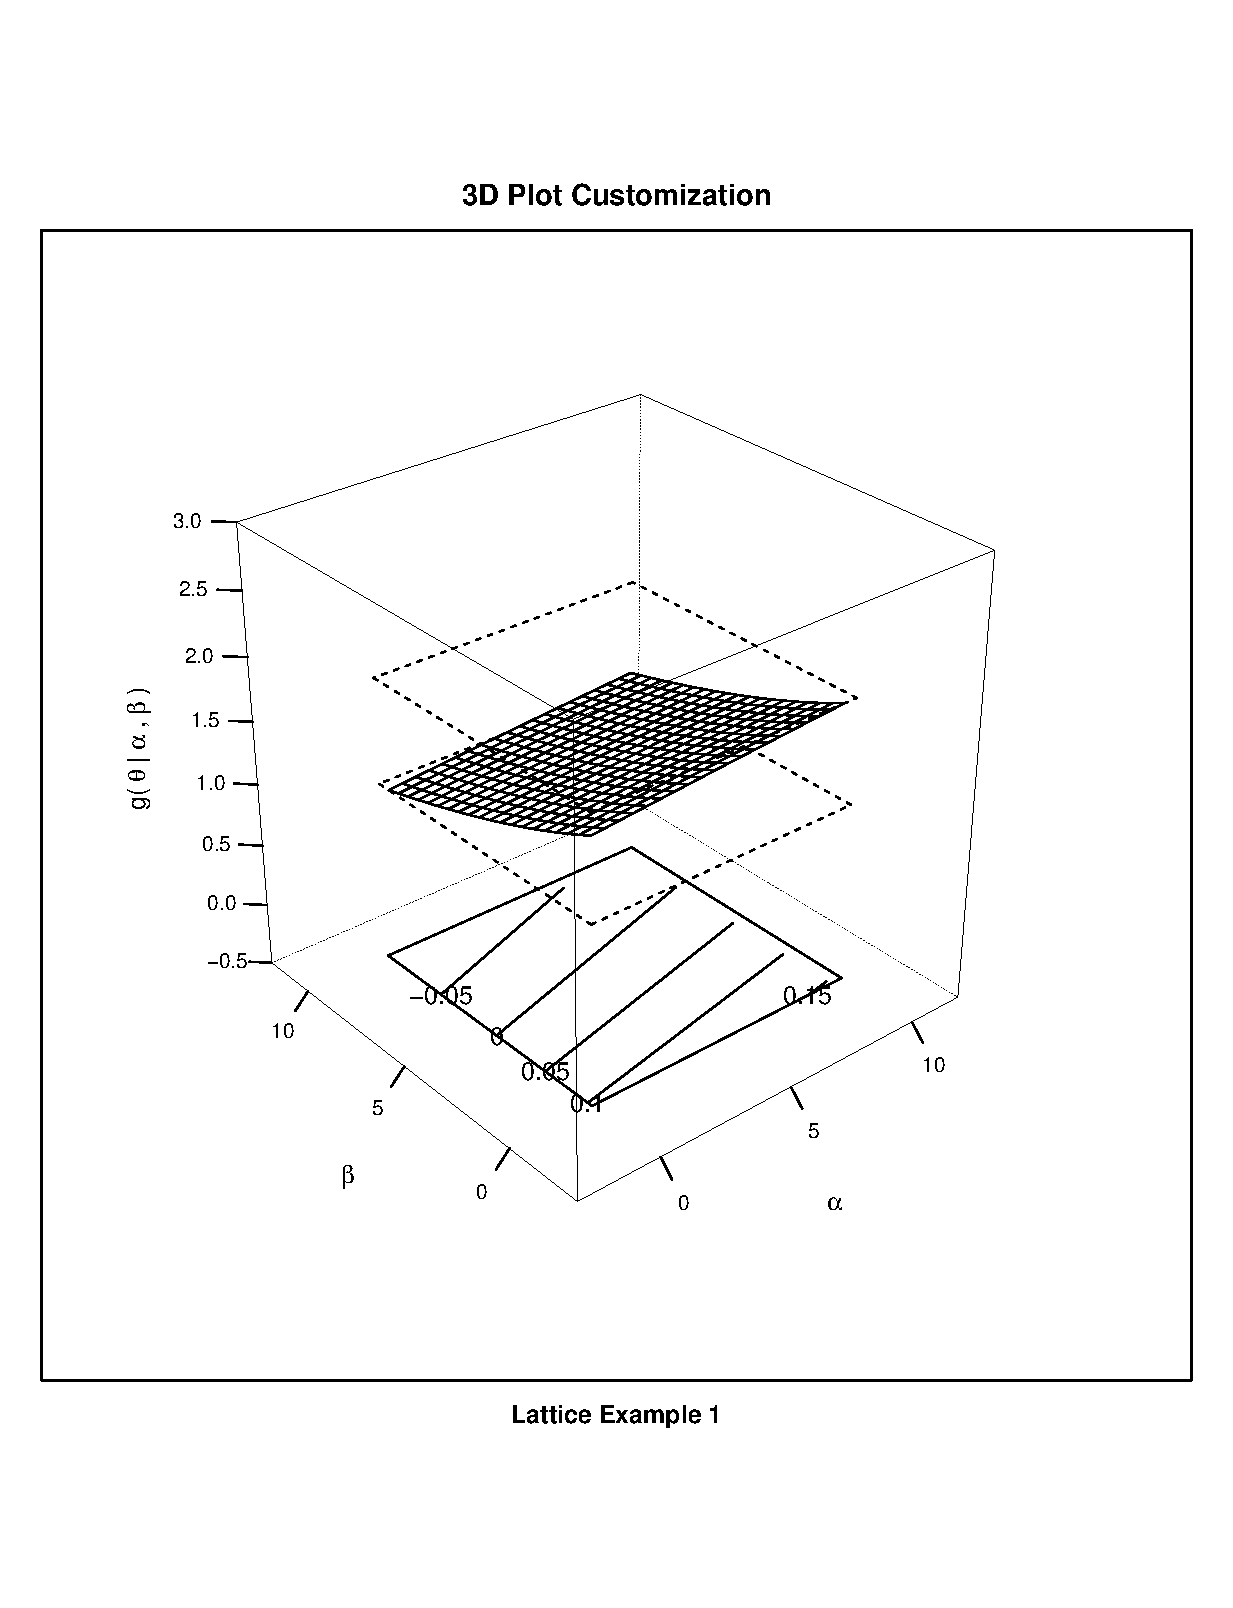
\includegraphics{./img/lattice-fig.eps}


\item \LaTeX 의 문서에 포함될 \texttt{.eps} 그래픽을 \texttt{R}에서 뽑았을 때는 아무런 문제가 없어 보였는데, 정작 \texttt{pdf}로 문서를 뽑아 보니까 이 그래픽이 들어간 페이지가 90도로 돌아가 있거나 혹은 그래픽이 90도로 회전되어 있을 경우에는 아래와 같이 하면 됩니다.

\begin{Schunk}
 \begin{Sinput}
  postscript(file=``filename.eps'', onefile=FALSE, horizontal=FALSE)
 \end{Sinput}
\end{Schunk}

이 문제에 대한 출처는 \texttt{postscript} 도움말입니다.

이문제를 다른 방법으로도 해결할 수 있습니다.  (대충 서너개 더 있음).

\item 새로운 그래픽 객체를 생성하는 방법을 설명해줘서 사용자가 추후에 독립적인 그래픽을 생성할 수 있게 도와주기 
\end{enumerate}

% ggplot2에서 stat_density2d에 오류가 있는것 같습니다. 모든 경우에 NA가 return된다는 보고




%%%%%%%%%%%%%%%%%%%%%%%%%%%%%%%%%%%%%%%%%%%%%%%%%%%%%%%%%%%%%%%%%%%%%%%%
%
% Utilities
%
%%%%%%%%%%%%%%%%%%%%%%%%%%%%%%%%%%%%%%%%%%%%%%%%%%%%%%%%%%%%%%%%%%%%%%%%

\chapter{데이터 입출력 및 파일관리 유틸리티}
\begin{enumerate}
\item \texttt{read.table} 계열의 함수를 이용하여 데이터를 불러올 때 첫번째 인자는 파일의 위치와 파일명이 입력된 문자열이어야 합니다.
그런데, 간혹 문법에서 틀린 점도 없고, 불러오고자 하는 데이터 파일도 올바른 파일경로에 위치하고 있음에도 불구하고,
데이터를 찾을 수 없다고 하는 경우가 있습니다.
이것은 내부적으로 파일경로에 띄어쓰기, 특수문자, 혹은 특수한 인코딩 등 다양한 이유로 인하여 파일경로가 올바르게 처리되지 않았기 때문입니다.
아래와 같은 방법으로 \texttt{read.table()} 함수 사용시 \texttt{file.choose()} 함수를 함께 사용하면 이러한 문제를 해결이 가능합니다.


\begin{Schunk}
\begin{Soutput}
mydata <- read.table(file.choose(), header=TRUE, sep=",")
\end{Soutput}
\end{Schunk}


\end{enumerate}




%%%%%%%%%%%%%%%%%%%%%%%%%%%%%%%%%%%%%%%%%%%%%%%%%%%%%%%%%%%%%%%%%%%%%%%%
%
% Miscellinous
%
%%%%%%%%%%%%%%%%%%%%%%%%%%%%%%%%%%%%%%%%%%%%%%%%%%%%%%%%%%%%%%%%%%%%%%%%

\chapter{클래스와 메소드 그리고 패키지 제작}
\begin{enumerate}
\item 패키지를 만들고 싶어요. (흠.. Generalized Linear Model 프레임워크 흉내내서 똑같이 만들어보기 실습자료로 제공해주기)
\end{enumerate}



%%%%%%%%%%%%%%%%%%%%%%%%%%%%%%%%%%%%%%%%%%%%%%%%%%%%%%%%%%%%%%%%%%%%%%%%
%
% Miscellinous
%
%%%%%%%%%%%%%%%%%%%%%%%%%%%%%%%%%%%%%%%%%%%%%%%%%%%%%%%%%%%%%%%%%%%%%%%%

\chapter{인코딩과 한글}

이 부분은 데이터를 불러오고 쓰는 방법과 연관되었으므로 해당 챕터로 이동시키는게 좋을 것 같음 (제안 수용됨)

\begin{enumerate}
\item 불러오고자 하는 데이터의 인코딩이 UTF-8가 아닐때 이를 확인하고, 데이터를 올바르게 불러오기 위한 내용은 \url{http://lists.r-forge.r-project.org/pipermail/ihelp-urquestion/2013-April/000017.html} 를 읽어보시길 바랍니다.

\item \texttt{R}을 한국어가 아닌 영문으로 사용하고 싶습니다 (버전에 관계없이 일반적으로 통용되는 방법 - 윈도우즈 사용자에게 맞추어 작성됨).
이를 설정하는 방법에 대해서는 \url{http://lists.r-forge.r-project.org/pipermail/ihelp-urquestion/2013-April/000003.html} 을 읽어보시길 바랍니다.
\end{enumerate}


%%%%%%%%%%%%%%%%%%%%%%%%%%%%%%%%%%%%%%%%%%%%%%%%%%%%%%%%%%%%%%%%%%%%%%%%
%
%
%
%%%%%%%%%%%%%%%%%%%%%%%%%%%%%%%%%%%%%%%%%%%%%%%%%%%%%%%%%%%%%%%%%%%%%%%%

\chapter{간단한 GUI 제작 해보기}

\begin{enumerate}
	\item 다른 언어로 인터페이싱 하는 방법마로, 그냥 \texttt{R}에서 주어지는 패키지를 이용해서 간단한 GUI 환경만들기
	\item 아마도... R Commander를 확장하는 방법을 예로 들면 좋을 것 같음
	\item 원리도 간단히 설명해주면 더욱 좋을 것 같음. 
\end{enumerate}


%%%%%%%%%%%%%%%%%%%%%%%%%%%%%%%%%%%%%%%%%%%%%%%%%%%%%%%%%%%%%%%%%%%%%%%%
%
%
%
%%%%%%%%%%%%%%%%%%%%%%%%%%%%%%%%%%%%%%%%%%%%%%%%%%%%%%%%%%%%%%%%%%%%%%%%


\chapter{답변되지 않을 수도 있는 질문들}

\begin{enumerate}
	\item (접수: 2013-04-18, Reproducibility=NA) R의 장점이자 단점이라고 생각되는 것 중에 하나가 엄청난 수의 패키지들임. 즉 어떤 분석을 하고자 할 때 그것에 대해 하나의 패키지가 있는 것이 아니라 대체적으로 사용가능한 패키지들이 존재하는데 이들 중 어느 것을 써야할 지 잘 모름. 다른 분석 프로그램의 경우 이러한 문제가 없는데... 결국엔 어떻게 제일 성능이 좋은? 결과가 신뢰할 만한? 좋은 패키지를 선택하는가를 알려주었으면 좋겠씀돠.
	
	\textsf{(답변)} 이것은 경험에 해당되며, 해당분야의 전문가로부터의 조언을 받는 것이 안전합니다.  그렇지 않다면, 직접 베이스를 이용하여 작성하면 됩니다. 
	
\end{enumerate}
\end{document}

% R을 사용해서 web 크롤링을 하는데 속도가 엄청 느리네요 scan() 함수를 쓰면 url로부터 html데이터를 받게 되는데 이것을 substring()함수와 regexprs()함수를 사용하여 적절히 데이터를 분해 하는 작업을 하는데 엄청느리네요. 원체느린거 같은데 혹시 해결방안 아시는분 게시나요?

% R에 있는 ggplot2 패키지를 이용해 얻은 얻은 plot그림을 웹에 보여주는 방법에 대해 아시는 분 계신가요?
 
